%%%%%%%%%%%%%%%%%%%%%%%%%%%%%%%%%%%%%%%%%%%%%%%%%%%%%%%%%%%%%%%%%%%%%%%%%%%%%%
%
% Section file included in main project file using \input{}
%
% Assumes that LaTeX2e macros and packages defined in cg_comp.sty are
%   available
%
%%%%%%%%%%%%%%%%%%%%%%%%%%%%%%%%%%%%%%%%%%%%%%%%%%%%%%%%%%%%%%%%%%%%%%%%%%%%%%

 \section{Classical Guitar Compensation\label{sct:comp}}

As we discussed in \sct{tot_freq_shift}, \eqn{error_tot} provides a guide to how to modify our prototypical classical guitar to improve the tone of the strings shown in \fig{shift_classicalguitar_ej45_null}. We noted that the bending stiffness and the increase in string tension due to fretting sharpen the pitch, but that we can flatten it with a positive saddle setback and negative nut setback. As in \fig{uncomp}, let's choose the guitar and string properties listed in \tbl{mcg_specs} and \tbl{string_specs}. In this case, \Fig{comp_dsdn} shows that increasing the saddle setback tends to rotate the pitch curve clockwise, and increasing the magnitude of the negative nut setback displaces the pitch curve almost uniformly downward. In this context --- referring to \eqn{error_tot} --- we follow \eqn{comp_approx} and choose $\Delta S = B_0\, X_0$ to compensate for stiffness, and then select $\Delta N = - \kappa\, X_0\, \overline{Q} / 2$, where $\overline{Q}$ is the average relative displacement over the first 12 frets. In this case, we estimate $\Delta S = 1.75$~mm, $\Delta N = -0.49$~mm for $d = 0$, and $\Delta N = -0.55$~mm for $d = 10$. The pitch curve shown in \fig{comp_est} illustrates the dramatic improvement in tone that can be obtained via classical guitar compensation.

\begin{figure}
    \centering
    \begin{subfigure}[b]{0.8\textwidth}
        \centering
        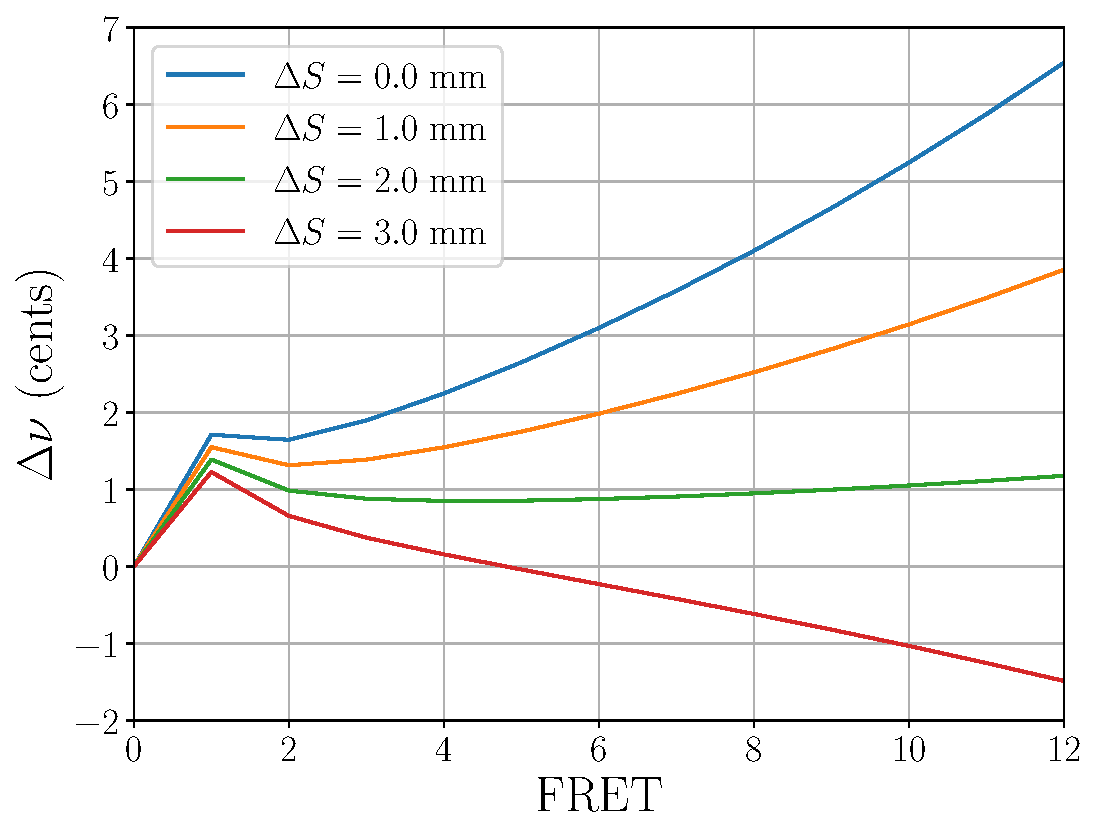
\includegraphics[width=5.0in]{../figures/comp_ds}
        \caption{Frequency shifts ($\Delta N = 0$)}
        \label{fig:comp_ds}
    \end{subfigure}
    \par\vspace{0.25in}
    \begin{subfigure}[b]{0.8\textwidth}
        \centering
        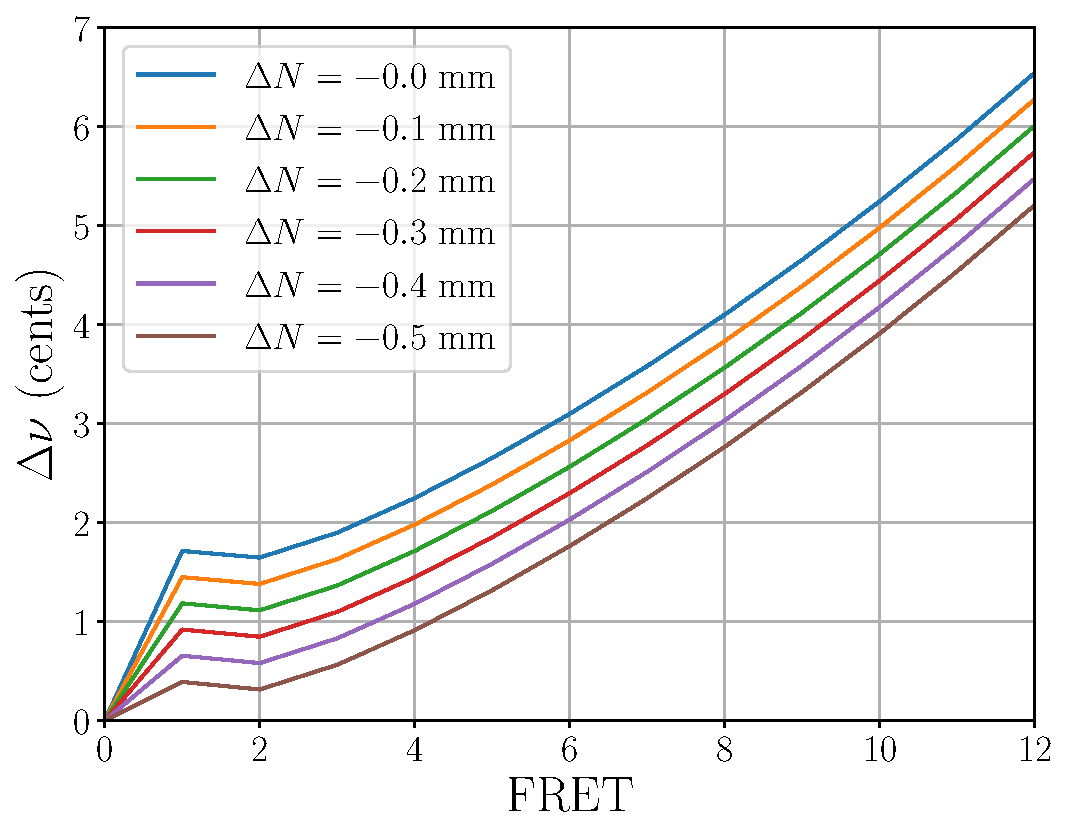
\includegraphics[width=5.0in]{../figures/comp_dn}
        \caption{Frequency shifts ($\Delta S = 0$)}
        \label{fig:comp_dn}
    \end{subfigure}
    \caption{\label{fig:comp_dsdn} In (a), we plot the frequency shifts for our classical guitar for several saddle setbacks with $\Delta N = 0$. Here $R = 24$ and the string radius is 0.5~mm. In (b), we set $\Delta S = 0$ and plot the frequency shifts for several nut ``setbacks.''}
  \end{figure}
  
  % \begin{figure}
  %   \centering
  %   \begin{subfigure}[b]{0.8\textwidth}
  %       \centering
  %       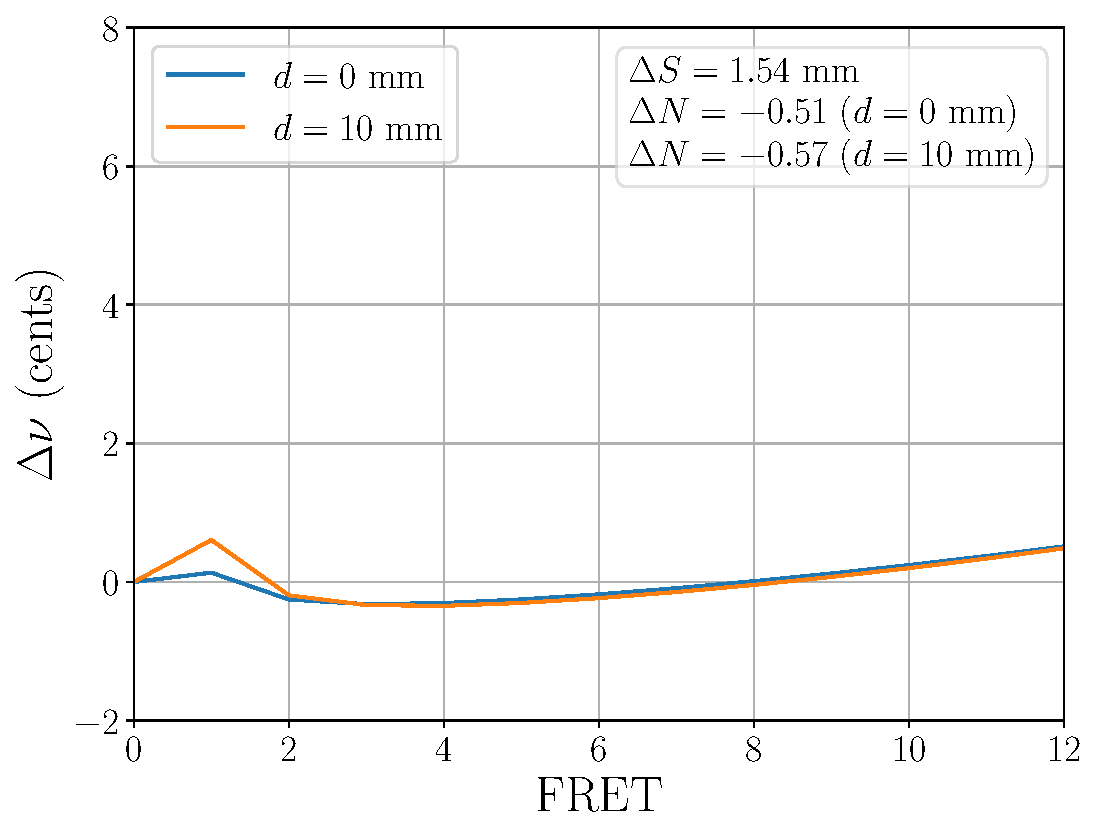
\includegraphics[width=5.0in]{../figures/comp_est}
  %       \caption{Approximate compensation}
  %       \label{fig:comp_est}
  %   \end{subfigure}
  %   \par\vspace{0.25in}
  %   \begin{subfigure}[b]{0.8\textwidth}
  %       \centering
  %       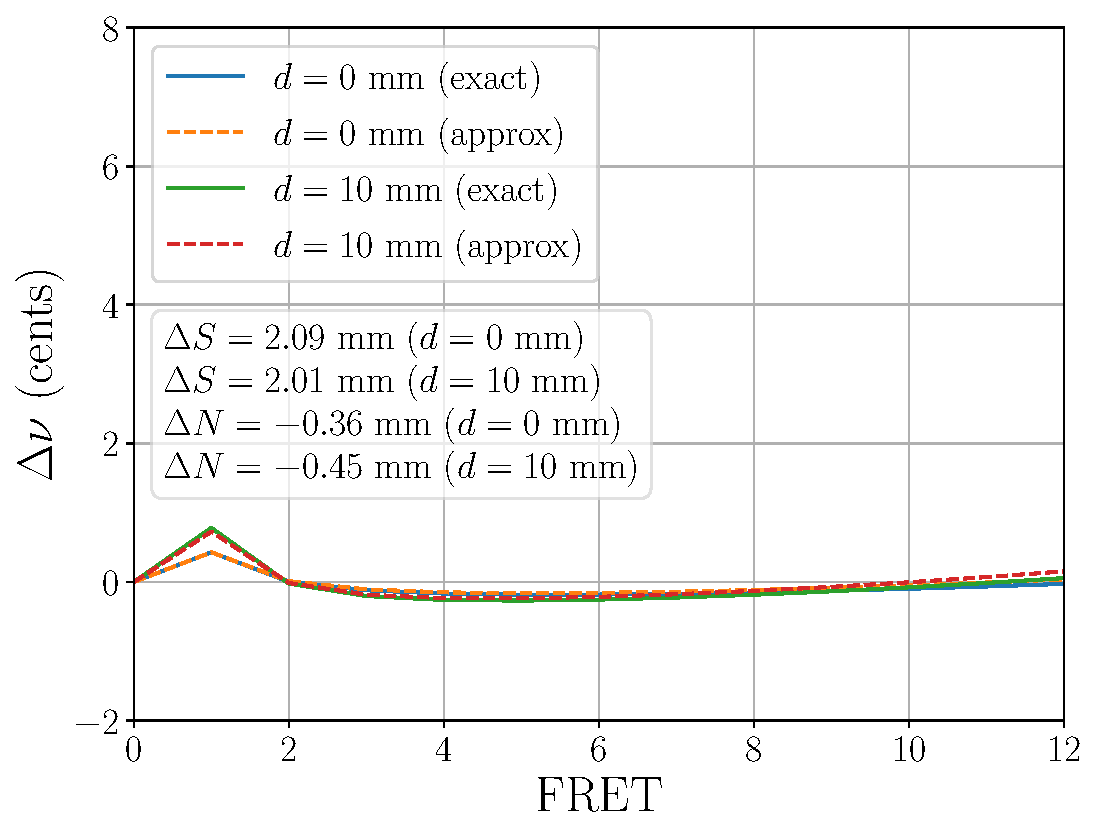
\includegraphics[width=5.0in]{../figures/comp_exact}
  %       \caption{Exact compensation}
  %       \label{fig:comp_exact}
  %   \end{subfigure}
  %   \caption{\label{fig:comp_model} In (a), we plot the frequency shifts for our classical guitar with approximate setbacks computed using \eqn{comp_approx}. In (b), we compute the same setbacks }
  % \end{figure}

\begin{figure}
  \centering
  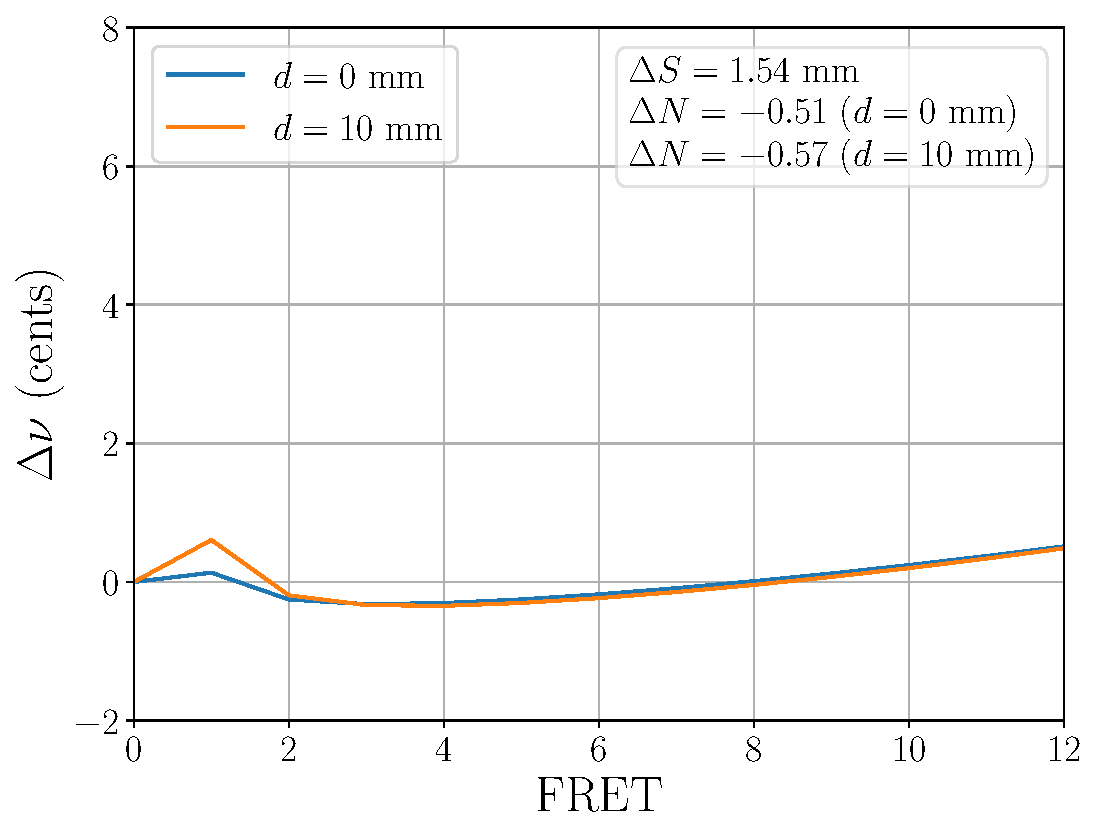
\includegraphics[width=5.0in]{../figures/comp_est}
  \caption{\label{fig:comp_est} The total frequency shift given by \eqn{error_def} for a classical guitar with a scale length of 650~mm, $b = 1.0$~mm, $c = 4.0$~mm, and a string with $R = 24$ and a radius $\rho = 0.5$~mm.}
\end{figure}

% Using the data and results presented in \tbl{ej45_props}, we can explore different approaches to compensating guitar strings for bending stiffness and string tension perturbations. For example, consider the guitar string shown in 

% For example, in \fig{shift_classicalguitar_ej45_factory}, using \eqn{error_def} we plot the frequency deviation (in cents) from ideal 12-TET for each string at each of the first 12 frets of an Alhambra 8P classical guitar, assuming that the open string has been perfectly tuned to the correct frequency. Recall that the Alhambra 8P is manufactured with a saddle setback of 1.5~mm, presumably to offset the effects of bending stiffness in the strings. For comparison, in \fig{shift_classicalguitar_ej45_null}, we plot the same deviations for the case where $\Delta S = 0$, which increases the error of each string at the 12$^\text{th}$ fret by 3 -- 4 cents. Recall from \sct{model} that we could crudely predict the values of the saddle and nut setbacks by inspecting \eqn{error_tot}. For example, from \tbl{ej45_props}, we estimate $\Delta S \approx B_0\, X_0 = 2.7$~mm and $\Delta N \approx -1.5$~mm for the third (G) string.

\begin{table}%[htbp]
  \centering
  \caption{\label{tbl:ej45_setbacks} Predicted setbacks for the D'Addario Pro-Arte Nylon Classical Guitar Strings -- Normal Tension (EJ45) on the Classical Guitar.}
  \begin{tabular}{cccc}
\toprule
String &  $\Delta S$ (mm) &  $\Delta N$ (mm) &  $\overline{\Delta \nu}_\text{rms}$ (cents) \\
\midrule
 J4501 &             2.16 &            -0.43 &                                        0.18 \\
 J4502 &             1.92 &            -0.31 &                                        0.15 \\
 J4503 &             4.36 &            -0.82 &                                        0.31 \\
 J4504 &             1.30 &            -0.19 &                                        0.13 \\
 J4505 &             1.94 &            -0.28 &                                        0.15 \\
 J4506 &             2.62 &            -0.35 &                                        0.16 \\
\bottomrule
\end{tabular}


\end{table}%

As an alternative to this simple approach, we adopt the method described in \app{rms} to compensate the Classical Guitar with normal tension nylon strings for the frequency errors shown in \fig{shift_classicalguitar_ej45_null}. Using \eqn{rms_sol_quad}, the setbacks we obtain for $d = 0$~mm are listed in \tbl{ej45_setbacks}, and the corresponding frequency deviations --- obtained with the listed setback for \emph{each} string --- are shown in \fig{shift_classicalguitar_ej45_full} (assuming that all other aspects of the guitar remain unchanged). Of course, manufacturing a guitar with unique saddle and nut setbacks for each string (of a particular tension) can be challenging, so we also plot in \fig{shift_classicalguitar_ej45_mean} the shifts obtained by setting each of the values of $\Delta S$ and $\Delta N$ to the mean of the corresponding column in  \tbl{ej45_setbacks}. In both cases, the RMS error is significantly smaller than that of the uncompensated guitar shown in \fig{shift_classicalguitar_ej45_null}. Note that the saddle setbacks tend to be larger --- and the nut setbacks smaller --- than the simple estimates that we made above for a hypothetical thick string. This is easily understood by examining \eqn{error_tot}: the portion of $\Delta S$ that exceeds $B_0\, X_0$ scales with $\gamma_n - 1$, and helps to compensate for tension errors as $n$ increases.

%  \begin{figure}
%   \centering
%   \begin{subfigure}[b]{0.8\textwidth}
%    \centering
%    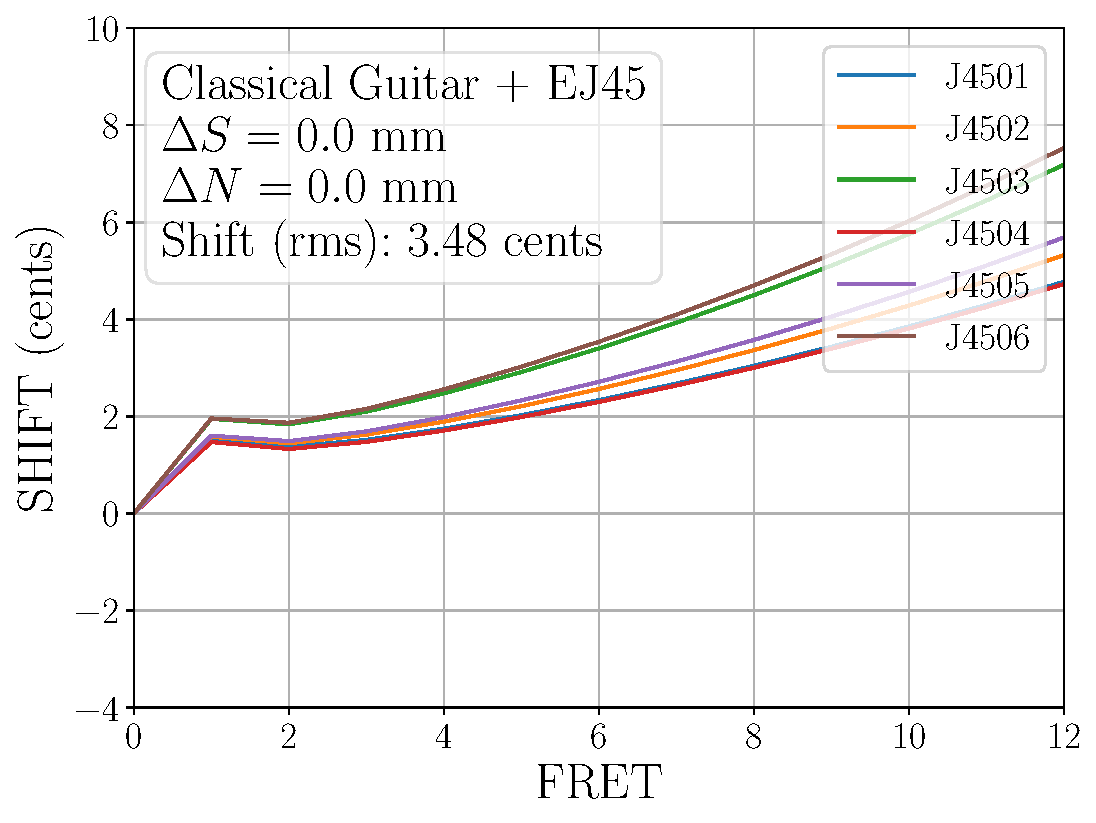
\includegraphics[width=5.0in]{../figures/shift_classicalguitar_ej45_factory}
%    \caption{Factory guitar}
%    \label{fig:shift_classicalguitar_ej45_factory}
%   \end{subfigure}
%   \par\vspace{0.25in}
%   \begin{subfigure}[b]{0.8\textwidth}
%    \centering
%    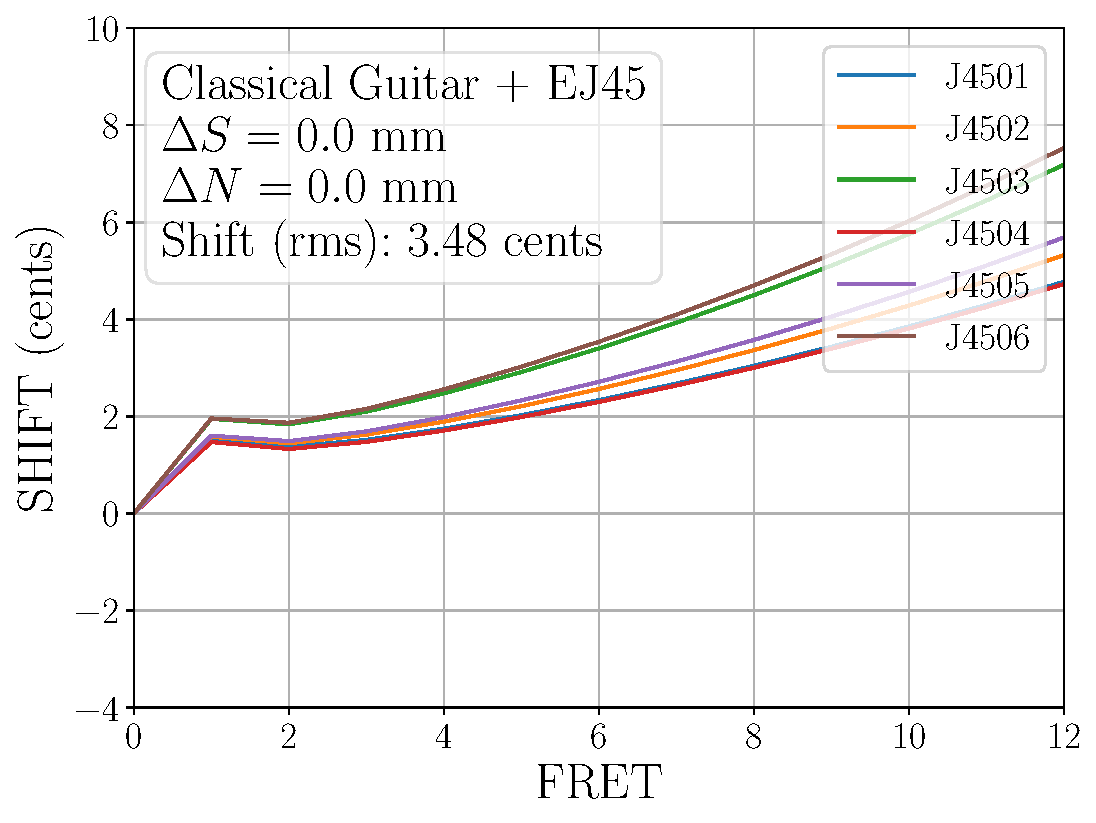
\includegraphics[width=5.0in]{../figures/shift_classicalguitar_ej45_null}
%    \caption{Uncompensated}
%    \label{fig:shift_classicalguitar_ej45_null}
%   \end{subfigure}
%   \caption{\label{fig:classicalguitar_ej45} Frequency shifts (in cents) for an Alhambra 8P guitar with normal tension nylon strings (D'Addario EJ45). In (a), we show the deviations of the guitar as manufactured in the factory, completely consistent with our measurements. In (b), we show the same 12-TET errors that would arise if $\Delta S = 0$ for the same guitar.}
%  \end{figure}

 \begin{figure}
  \centering
  \begin{subfigure}[b]{0.8\textwidth}
   \centering
   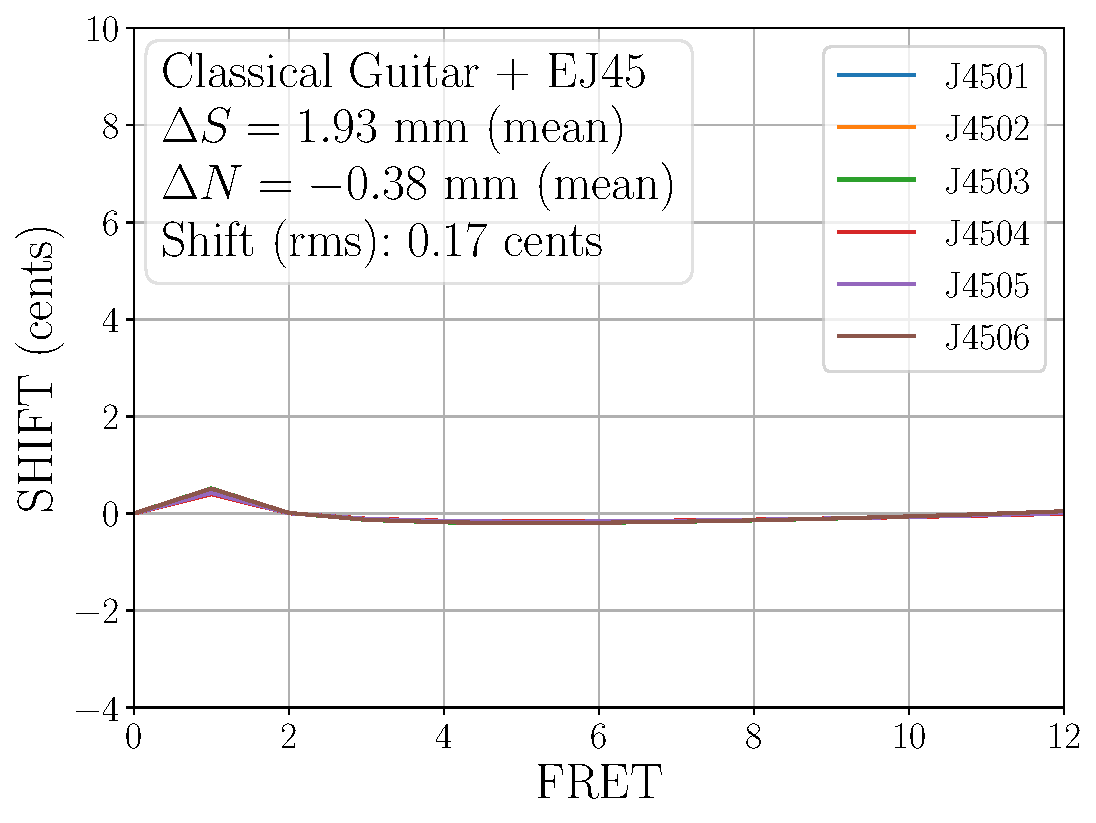
\includegraphics[width=5.0in]{../figures/shift_classicalguitar_ej45_full}
   \caption{Full compensation}
   \label{fig:shift_classicalguitar_ej45_full}
  \end{subfigure}
  \par\vspace{0.25in}
  \begin{subfigure}[b]{0.8\textwidth}
   \centering
   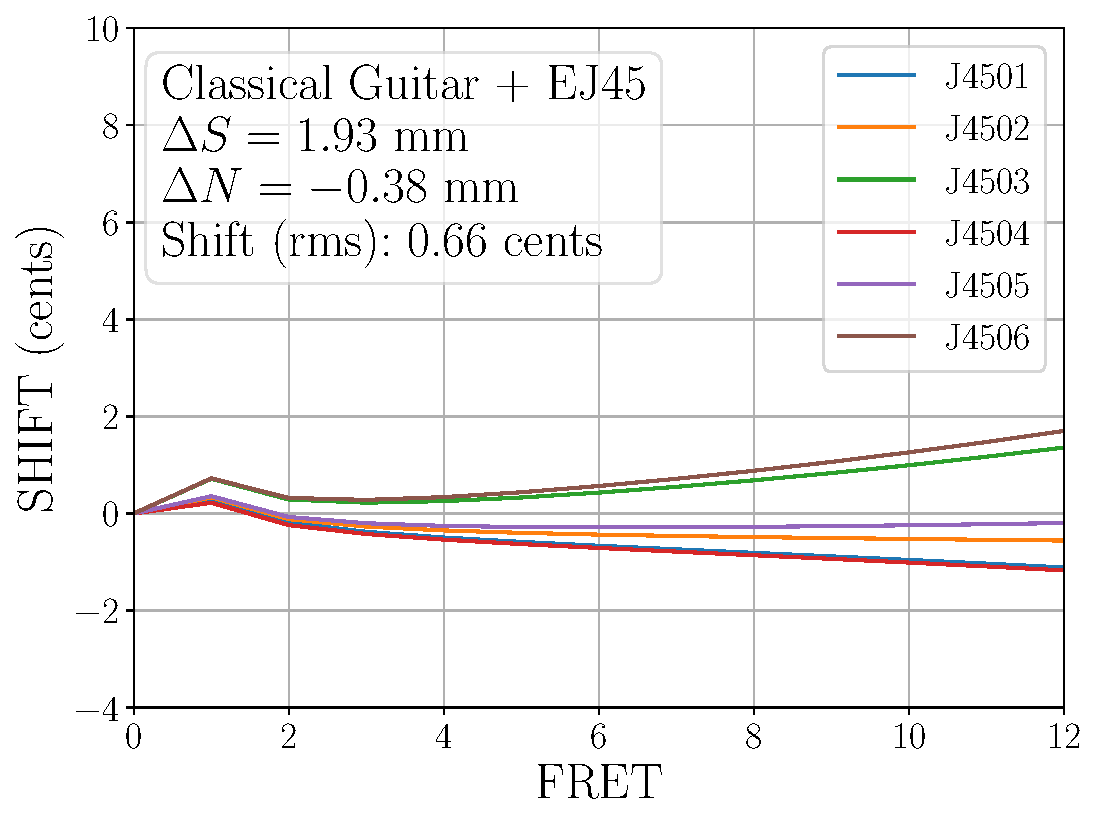
\includegraphics[width=5.0in]{../figures/shift_classicalguitar_ej45_mean}
   \caption{Mean compensation}
   \label{fig:shift_classicalguitar_ej45_mean}
  \end{subfigure}
  \caption{\label{fig:compensation_classicalguitar_ej45} Frequency shifts (in cents) for a classical guitar with normal tension nylon strings (D'Addario EJ45). In (a) we use the individual values for each string that are listed in \tbl{ej45_setbacks}. In (b), we set $\Delta S$ and $\Delta N$ to the mean of the corresponding column in that table.}
 \end{figure}

There are several other aspects of classical guitar compensation that are notable. First, as mentioned above, it is nontrivial to manufacture a guitar with different setbacks for each string~\cite{ref:byers1996cgi}, and it is unlikely that the exact values listed in \tbl{ej45_setbacks} are applicable to other string sets. We have measured the values of $R$ for five other string sets (with $d = 0$), and in \app{specs} we have reproduced the exact compensation procedure for them that we performed above for normal tension strings. Although each set exhibits variation between strings (and with respect to other sets) in individual setbacks for each string, they are similar enough that we suspect that there is the potential for great simplification in guitar design. For example, following the analysis of \app{rms}, it is possible to determine a single setback pair $\{\Delta S, \Delta N\}$ that minimizes the RMS frequency errors of an ensemble of strings over a collection of frets simply by computing the mean of the setbacks over all strings, and then using these mean values when manufacturing the guitar. If we consider five of the six string sets we have measured here --- neglecting the light tension strings because of their pathologically high values of $R$ --- we obtain the global mean setbacks $\Delta S = 1.90$~mm and $\Delta N = -0.38$~mm (when $d = 0$) for the saddle and nut, respectively. Note that these results are remarkably similar to the values used in \fig{shift_classicalguitar_ej45_mean}; if we plot the frequency deviations of those five string sets with these particular setback values, then we find that the maximum error always occurs at the twelfth fret, and it is always less than 2~cents. In the next section, we discuss a method to temper the guitar to reduce these errors further.

Second, after paying close attention to the impact of the act of fretting on our approximations in \sct{model}, we have simply set $d = 0$ in this section. This is because nonzero values of $d$ have an impact on the frequency deviation of a string at the first fret, and are otherwise negligible. This tends to increase the required mean value of the nut setback, but does not require a significant change to the saddle setback. As an example, in \fig{dsdnd_ej45}, we plot the mean optimum saddle and nut setbacks for the classical guitar parameters used in \fig{shift_classicalguitar_ej45_mean} with the D'Addario Nylon Normal Tension EJ45 string set as a function of the fretting distance $d$. Paying careful attention to the $y$-axis of these plots, we see that the value of the mean saddle setback \emph{decreases} by less than 5\% as $d$ increases to 10~mm, and the magnitude of the nut setback increases by almost 30\% at the same fretting offset. This behavior is essentially the same for all string sets considered in this work, and can be used by the luthier to determine the optimum setback values for their designs. Note that --- when the RMS approach is used to compute the mean setbacks --- the difference $\Delta S - \Delta N$ (the sum of the saddle setback and the magnitude of the nut setback) is virtually independent of $d$, as shown in \fig{dsnd_ej45}. We see here that the distance between the saddle and the nut \emph{does not depend on} $d$; as $d$ increases, the saddle and the nut move together toward the guitar bridge at lower $x$ values. Therefore, for values of $b$ and $c$ that are within 50\% of those listed in \tbl{mcg_specs}, we can fit the change of $\Delta N$ to a polynomial in $d/X_0$, and find
\begin{align} \label{eqn:comp_d_poly}
  \Delta N(d) &\approx \Delta N(0) \left[ 1 + 13\, (d/X_0) + 280\, (d/X_0)^2 \right]\, , \nd \\
  \Delta S(d) &\approx \Delta S(0) + \Delta N(0) \left[13\, (d/X_0) + 280\, (d/X_0)^2 \right]\, .
\end{align}
As $d$ increases, the magnitude of the negative nut setback increases, and the saddle setback decreases because $\Delta N < 0$. Updating the guitar string illustrated in \fig{comp_est}, and using both \eqn{rms_sol_quad} with \emph{no} approximations (``exact'') and \eqn{rms_sol_comp} with \eqn{comp_d_poly} (``approx''), we find the setbacks and show the corresponding frequency deviations in \fig{comp_exact}. The setback values computed using these two methods are virtually identical.

\begin{figure}
  \centering
  \begin{subfigure}[b]{0.8\textwidth}
      \centering
      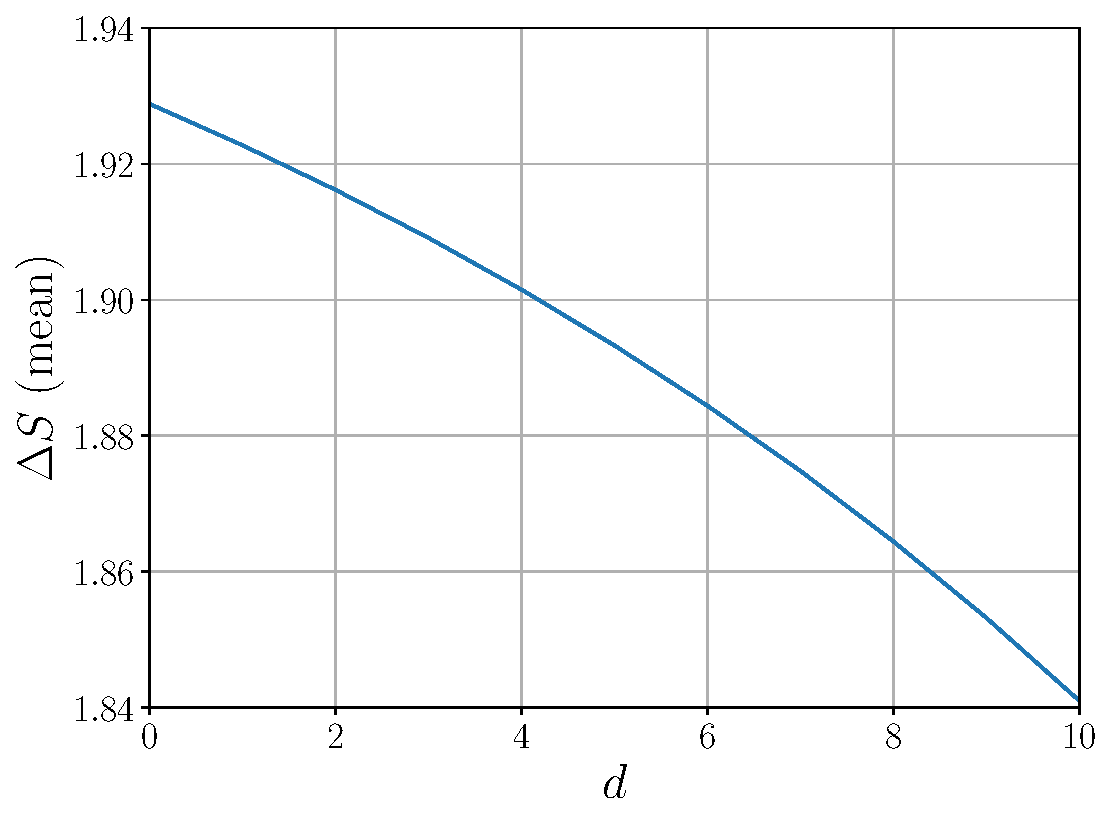
\includegraphics[width=5.0in]{../figures/dsd_ej45}
      \caption{Mean saddle setback}
      \label{fig:dsd_ej45}
  \end{subfigure}
  \par\vspace{0.25in}
  \begin{subfigure}[b]{0.8\textwidth}
      \centering
      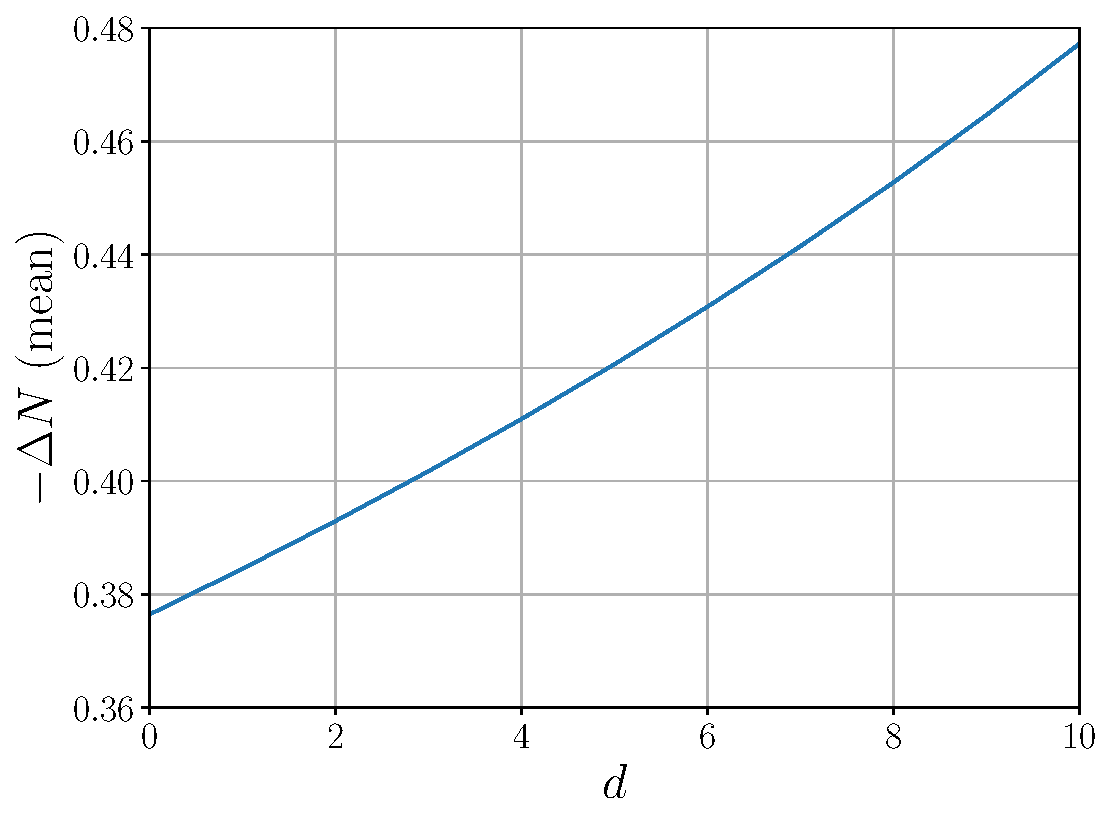
\includegraphics[width=5.0in]{../figures/dnd_ej45}
      \caption{Mean nut setback}
      \label{fig:dnd_ej45}
  \end{subfigure}
  \caption{\label{fig:dsdnd_ej45} The mean optimum saddle and nut setbacks for the D'Addario Nylon Normal Tension EJ45 string set as a function of the fretting distance $d$.}
\end{figure}

\begin{figure}
  \centering
  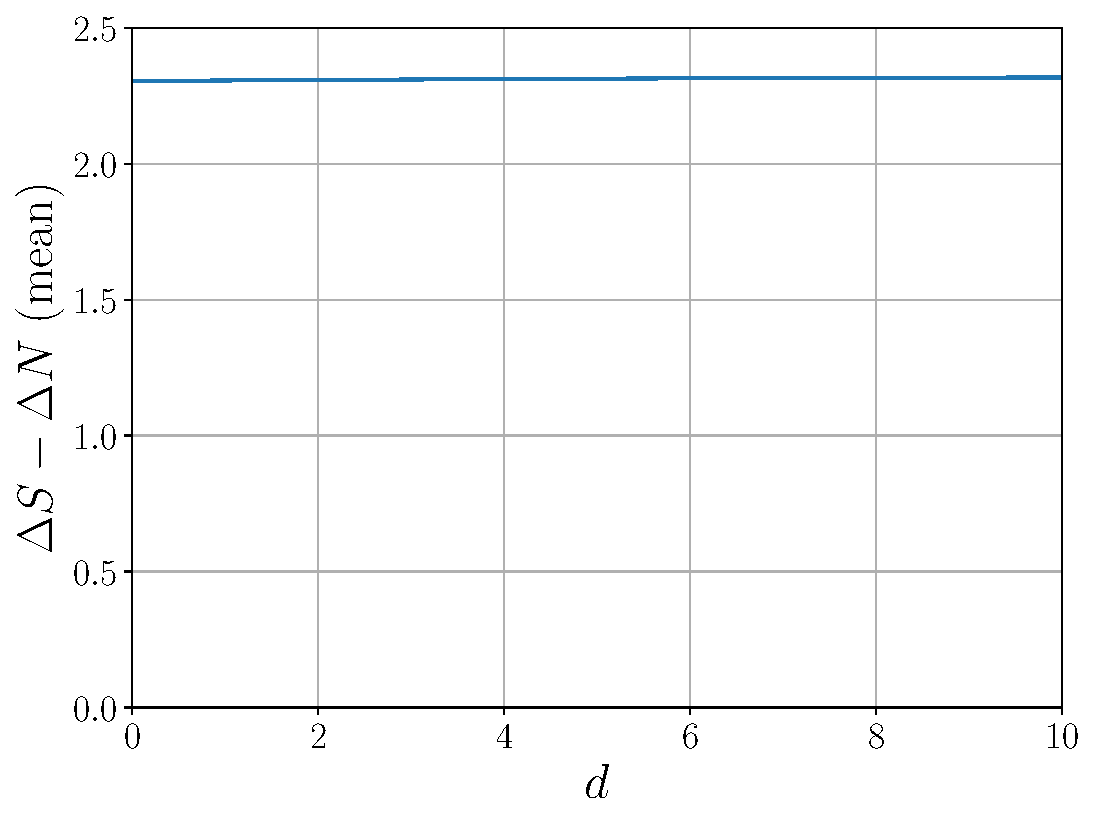
\includegraphics[width=5.0in]{../figures/dsnd_ej45}
  \caption{\label{fig:dsnd_ej45} The mean value of $\Delta S - \Delta N$ for the D'Addario Nylon Normal Tension EJ45 string set as a function of the fretting distance $d$.}
\end{figure}

\begin{figure}
  \centering
  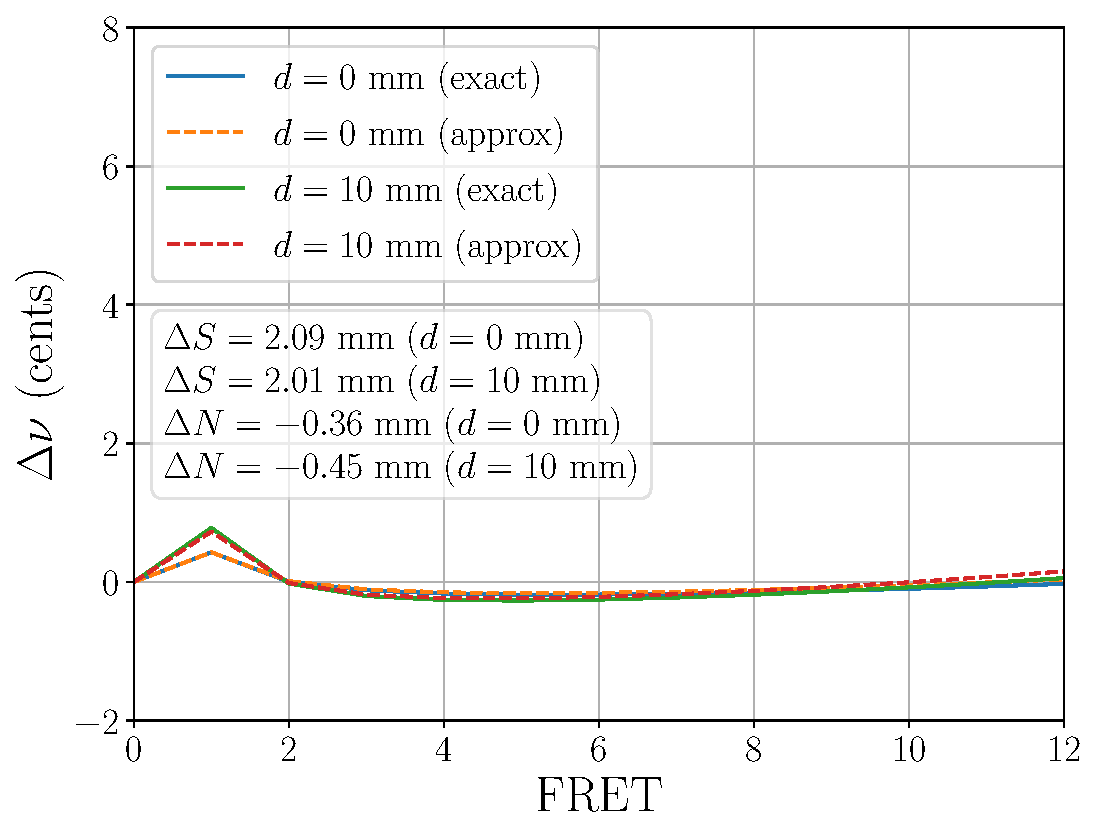
\includegraphics[width=5.0in]{../figures/comp_exact}
  \caption{\label{fig:comp_exact} The total frequency shift given by \eqn{error_def} for a classical guitar with setbacks computed using both \eqn{rms_sol_quad} with \emph{no} approximations (``exact'') and \eqn{rms_sol_comp} with \eqn{comp_d_poly} (``approx'').}
\end{figure}

\begin{figure}
  \centering
  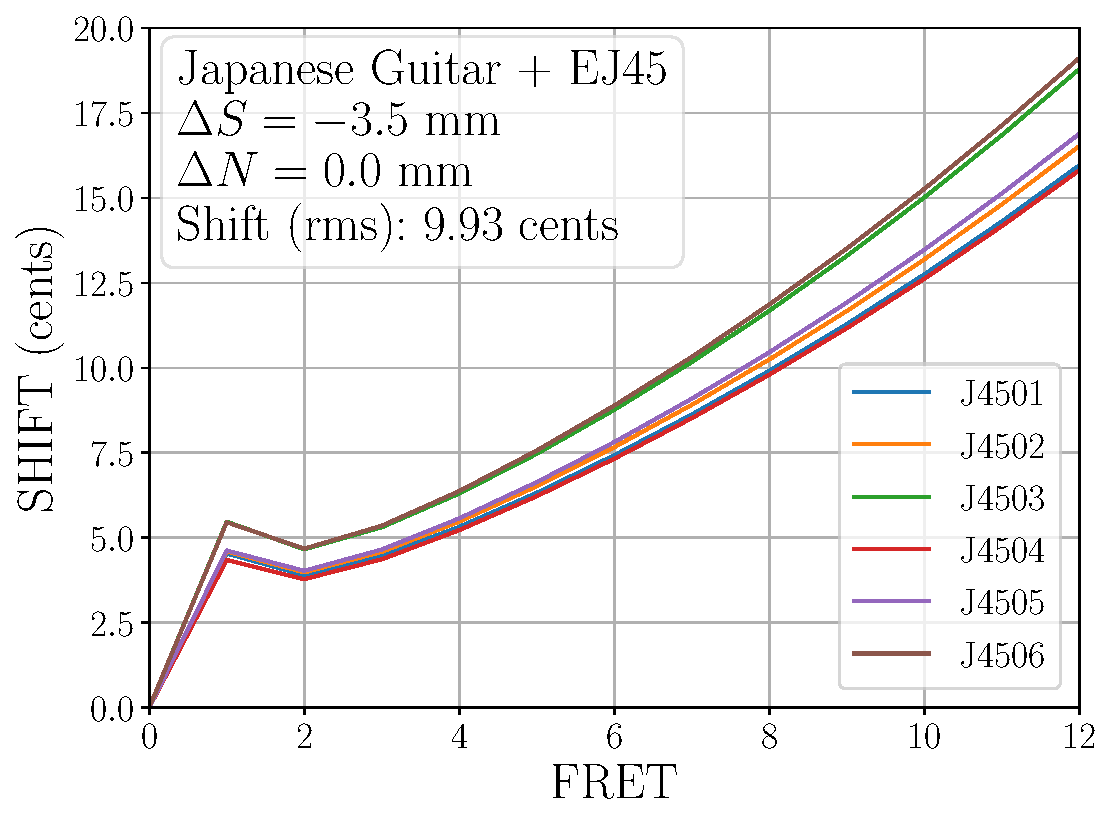
\includegraphics[width=5.0in]{../figures/japan_guitar_ej45_shifts}
  \caption{\label{fig:japan_guitar_ej45_shifts} Frequency shifts for a classical guitar using normal-tension nylon strings with $b = 1.4$~mm, $c = 5.5$~mm, $d = 10$~mm, $X_0 = 652$~mm, $\Delta S = -3.5$~mm, and $\Delta N = 0$~mm. The points represent the measurement data, while the lines are predictions made using \eqn{error_def}.}
\end{figure}

Third, recall that we recalculated the expected frequency shift of a classical guitar string with asymmetric boundary conditions in \app{freq}, and found an expression for $f_q$ given by \eqn{f_m_hybrid} that reduces --- by about a factor of 2 --- the impact of the bending stiffness relative to the symmetric (clamped) case in \eqn{f_m_clamped}. Furthermore, we have not used more sophisticated techniques to calculate the bending stiffness for either monofilament nylon strings or wound nylon strings, opting instead for the phenomenological model given by \eqn{b_0_kappa}. But is this approach valid? As a test, we compared our frequency shift estimates based on \sct{model} with experimental measurements made using a guitar manufactured in Japan with a few unique design choices: $b = 1.4$~mm, $c = 5.5$~mm, $d = 10$~mm, $X_0 = 652$~mm, $\Delta S = -3.5$~mm, and $\Delta N = 0$~mm. The larger value of $b$ and the large \emph{negative} saddle setback result in very large frequency deviations at all frets. As shown in \fig{japan_guitar_ej45_shifts}, we measured the shifts at the first fret and found that they fell into the range of $4.5 - 5.75$~cents, consistent with our predictions. At the 12$^\mathrm{th}$ fret, we measured $\Delta f = 18.5 - 19.5$~cents for the third and sixth strings, and $\Delta f = 15.75 - 17.5$~cents for the other strings, in reasonably close agreement with our predictions. By contrast, the corresponding equation arising from symmetric (clamped) boundary conditions --- \eqn{f_m_clamped} --- predicts shifts that are $30 - 45$\% higher, and setbacks that are more than a factor of two larger. We conclude that \eqn{f_m_hybrid} and \eqn{b_0_kappa} can be used to reliably predict setbacks for classical guitars.

Finally, many luthiers provide ``relief'' to enlarge the effective height of the string (particularly for the wound bass strings) as the fret number grows to provide clearance for vibration amplitude at higher volume. In practice, this is accomplished by pivoting the fret board shown in \fig{guitar_schematic} clockwise about $x = X_0$, increasing the height of the string above fret $n$ by an amount
\begin{equation}
  \begin{split}
    \Delta y_n &= m \left(X_0 - X_n\right) \\
    &= \frac{\gamma_n - 1}{\gamma_n}\, m\, X_0 \\
    &= \frac{\gamma_n - 1}{\gamma_n}\, 2\, \Delta y_{12}\, ,
  \end{split}
\end{equation}
where $\Delta y_{12}$ is the relief at the twelfth fret and $m = 2\, \Delta y_{12} / X_0 \ge 0$ is the downward slope of the fret board. If we update \eqn{l_n_def} and \eqn{l_p_def} (with $d = 0$), then we obtain
\begin{subequations}
  \begin{align}
    L_n &= \sqrt{\left(X_n + \Delta S\right)^2 + (b + \Delta y_n + c)^2}\, , \nd \\
    L^\prime_n &= \sqrt{\left(X_0 - X_n + \Delta N\right)^2 + \left(b + \Delta y_n\right)^2}\, .
  \end{align}
\end{subequations}
These equations indicate that we could update the approximation for $Q_n$ given by \eqn{q_n_approx} by replacing $b \longrightarrow b + \Delta y_n$, which results in the numerator
\begin{equation}
  \gamma_n\, b + (\gamma_n - 1)\, c \longrightarrow \gamma_n\, b + (\gamma_n - 1) \left(c + 2\, \Delta y_{12}\right)\, ,
\end{equation}
indicating that the intuitive substitution $c \longrightarrow c + 2\, \Delta y_{12}$ in \eqn{q_n_approx} captures the effect of relief. (Note that this should \emph{not} be done when computing the length $L_0$ of the open string!)
